% !TEX root = thesis-ex.tex
Of the different jet reconstruction algorithms that were discussed in Section~\ref{sec:jet_algo}, the LHC collaborations use the \antikt\ algorithm.
The ATLAS jet reconstruction procedure in heavy ion collisions is summarized in Figure~\ref{fig:atlasHIjetreco}.

\begin{figure}[htbp!]
	\centering
	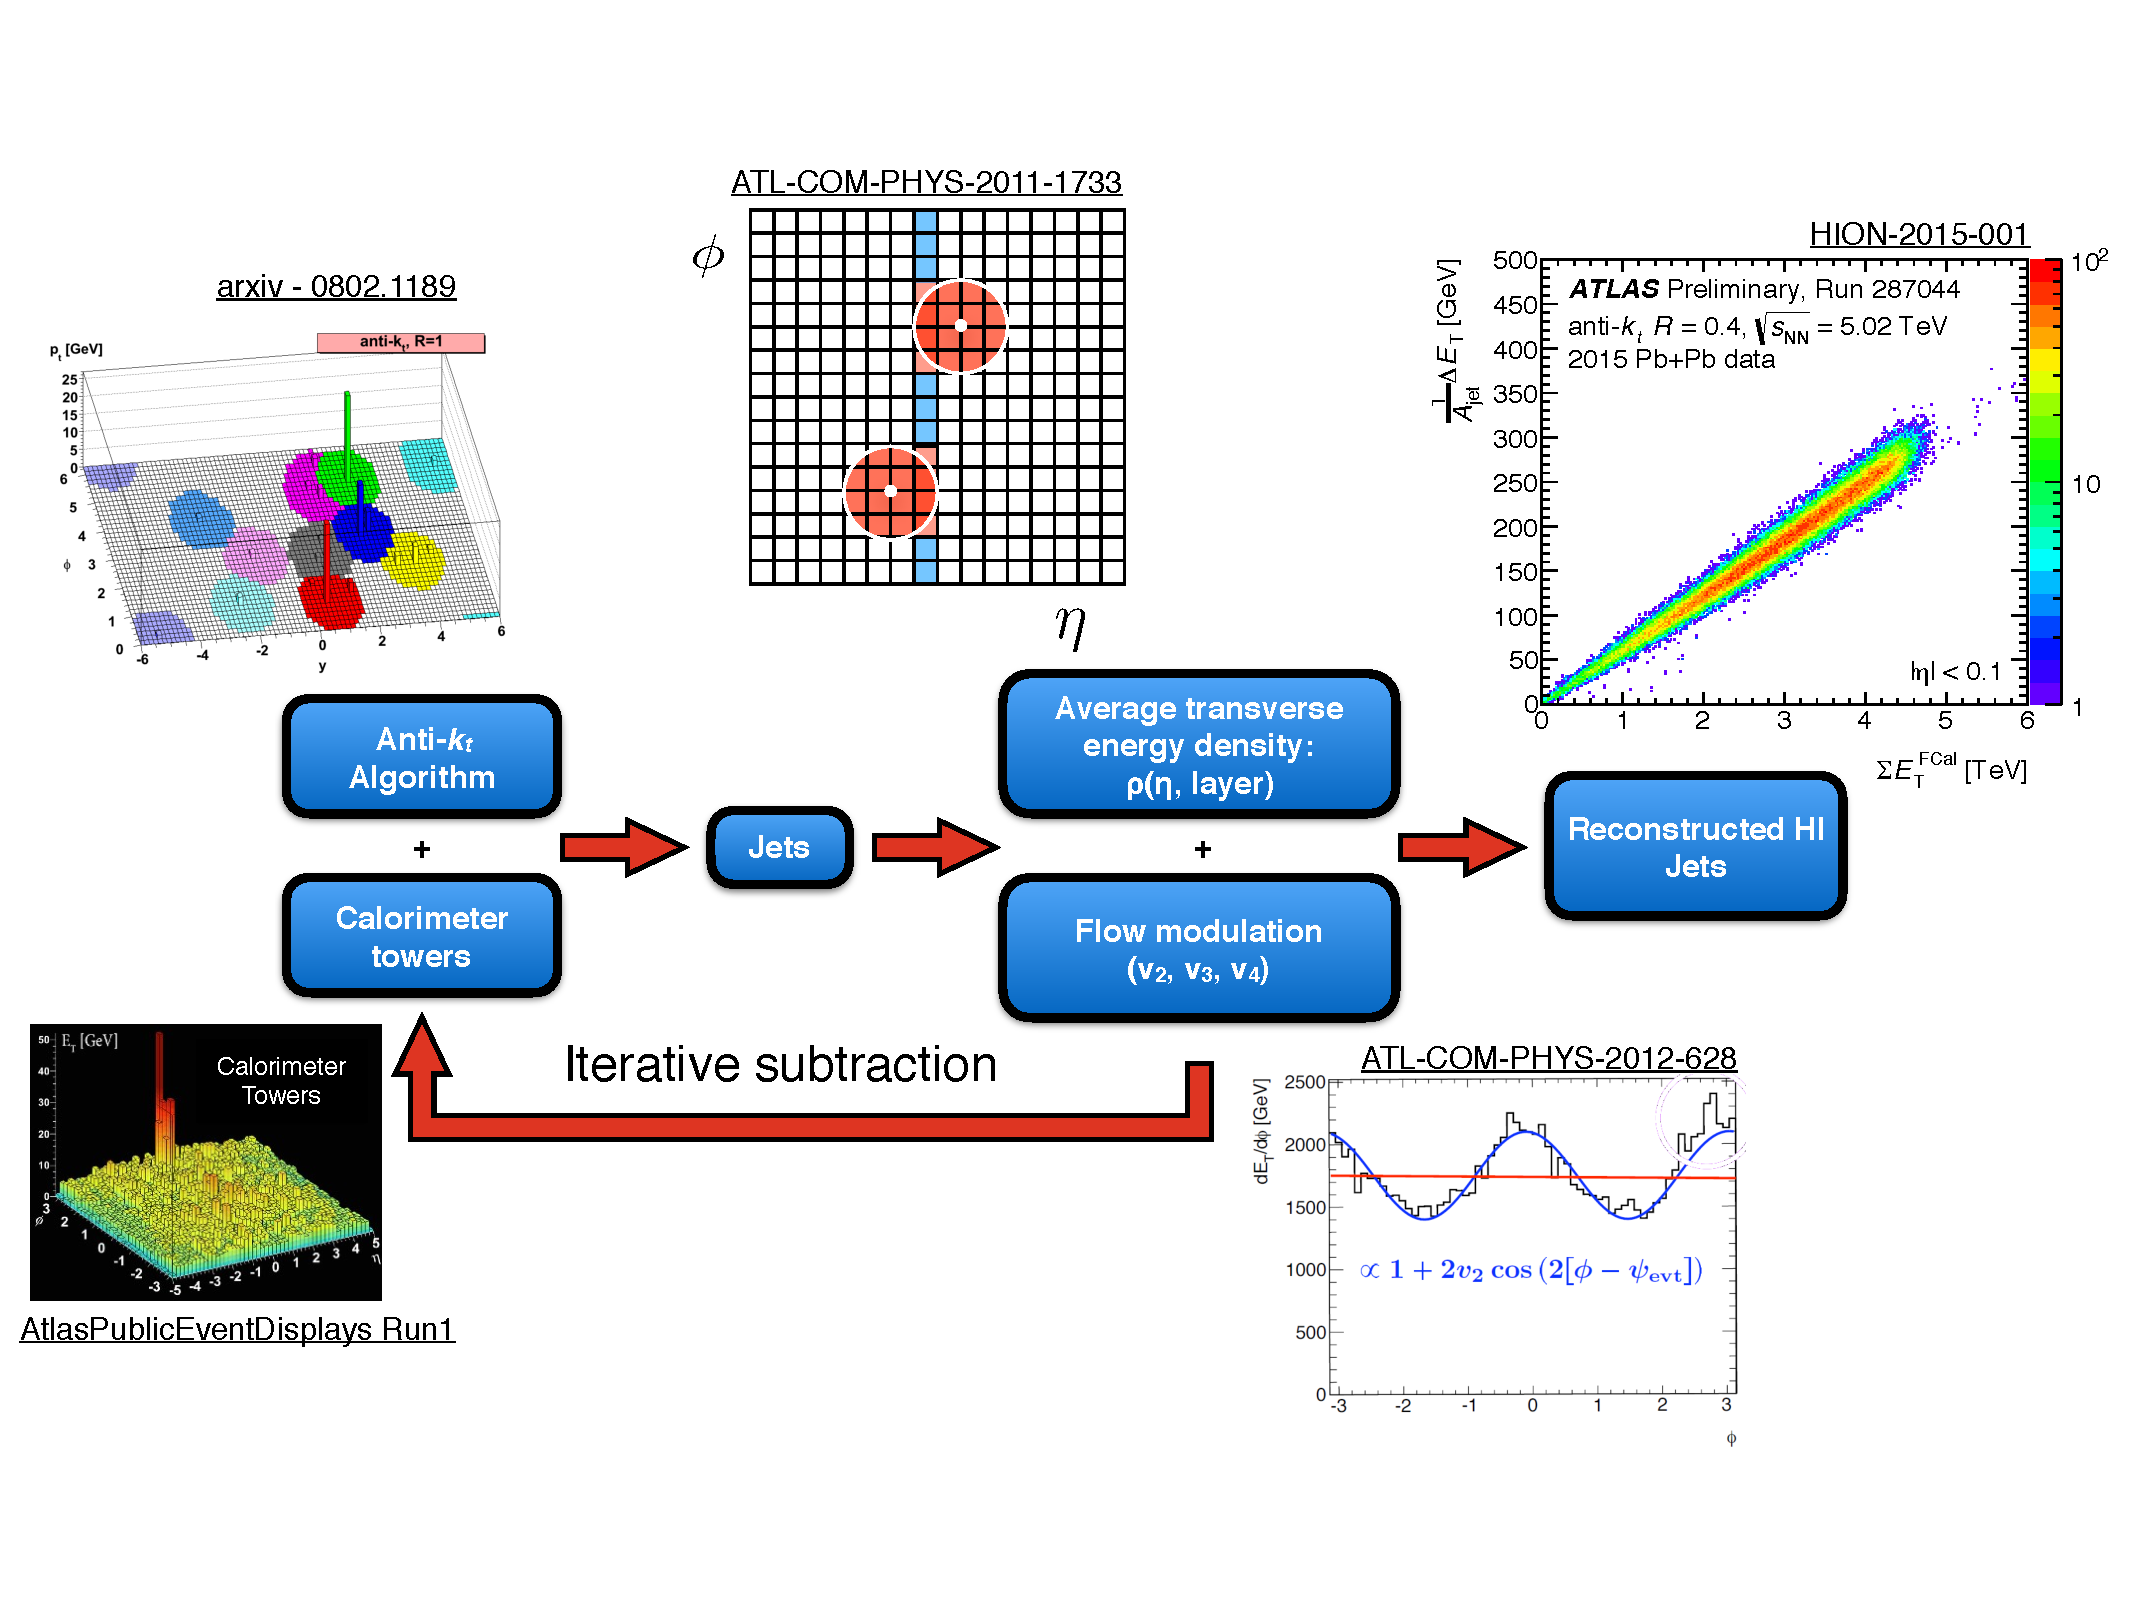
\includegraphics[width=\textwidth]{figures/setup/atlasHIjetReco} %
	\caption{A schematic of the ATLAS jet reconstruction procedure.
	Figures taken from \cite{Cacciari:2008gp, atlasRun1EventDisplay, ATLAS-COM-PHYS-2011-1733, Cole:1450219, perfPlots}.}	
	\label{fig:atlasHIjetreco}%
\end{figure}

This procedure uses the \antikt\ algorithm as implemented in \textsc{FastJet} software package \cite{fastjet_algo}.
The \antikt\ algorithm is run in four-momentum recombination mode with its inputs being the $\eta \times \phi = 0.1 \times \pi / 32$ calorimeter towers.
The tower energies are the sum of the energies of all layers in the tower with cells that straddle tower boundaries having their energies fractionally distributed.
The \antikt\ algorithm is first run with the distance parameter $R=0.2$, following which an underlying event subtraction procedure is performed.
A first estimate of the average underlying event energy density $\rho_i (\eta)$ is done in 0.1 slices of $\eta$ in each calorimeter layer $i$ after excluding the regions that overlap with the seed jets.
These seed jets are defined as jets having $R = 0.2$ and containing at least one tower with $\Et > 3$ GeV.
The ratio of the maximum tower transverse energy to the average tower transverse energy ($\Et^{Max} / \langle \Et \rangle$) should be at least 4.
A modulation is applied to account for the flow from the QGP (discussed in Section~\ref{sec:qgp}) and the underlying event is subtracted to give $E_{Tj}^{\mathrm{sub}}$:

\begin{align}
E_{Tj}^{\mathrm{sub}} = E_{Tj} - A_j \rho_i (\eta_j) \Big(1+2 \sum_{n=2}^{4} {v_{n}}_i \big(\cos[2(\phi-\Psi_n)] \big) \Big)
\end{align}
where $E_{Tj} , \eta_j, \phi_j$ and $A_j$ are the cell $E_T, \eta, \phi$ and area for cell $j$ in layer $i$.
$\Psi_n$ is the event plane angle and is given by:

\begin{align}
\Psi_n = \frac{1}{n} \tan^{-1} \left[ \frac{\langle \sum_k w_k \Et_k \sin(n\phi_k) \rangle}{\sum_k \Et_k \sin(n\phi_k)} \right]
\end{align}
where the sum is over all $k$ cells in the FCal. $\phi_k$ is the azimuthal angle of the cell and $w_k$ is a weight assigned to each cell to ensure a uniform $\Psi_n$ distribution. 
The dominant effect in the modulation is from the second and third harmonic, $v_2$ and $v_3$ \cite{ATLAS:2012at}.
These are given by:

\begin{align}
v_{ni} = \frac{\sum_{j \in i} \Et_j \cos[2(\phi-\Psi_n)]}{\sum_{j \in i} \Et_j}
\end{align}
where the sum is over all cells $j$ in layer $i$.

This subtraction process is iteratively done one more time after getting new seeds with the distance parameter $R = 0.2$ and excluding areas that are within $\Delta R = 0.4$ of the seeds.
Updated values of $\rho{'}_i$ and $v{'}_2$ are recalculated and used to estimate the background that is subtracted from the original cell energies.
This is then subtracted from the original cell energies to give kinematics for the $R= 0.4$ jets.

These jets still require a calibration before they can be used for analysis.
This is done via an Monte-Carlo (MC) based procedure.
\subparagraph{add cross calirbation stuff bere}
The performance of the jet reconstruction is tested by evaluating the jet energy scale and jet energy resolution.
These are the mean and width respectively of the jet response distribution that is given by $\ptreco / \pttruth$ in MC.
\ptreco\ is the reconstructed jets transverse momentum, while \pttruth\ is the transverse momentum of the corresponding ``truth'' jet from a MC generator such as \pythia8.

add parametrization of jer (https://www.sciencedirect.com/science/article/pii/S037026931830995X#br0410)


More details on this procedure can be found in \cite{2013220}.




